\appendix

\section{Appendiks - Forklaring på segfault}\label{app:segfault}

Når dere kompilerer et program, vil dere til slutt ende opp med noe som ligner på figur \ref{fig:4-minne-struktur}. Programmet er delt opp i områder med forskjellige rettigheter. Feltet \verb|.text| er minne-området som inneholder maskinkoden som faktisk kjører, samt statisk lenkede biblioteker. Dette området krever lese- og kjørerettigheter, men vi har virkelig ikke lyst til å gi området skriverettigheter - fordi programmet da potensielt kunne ha skrevet om seg selv.

\begin{figure}[ht]
    \centering
    

\tikzset{every picture/.style={line width=0.75pt}} %set default line width to 0.75pt        

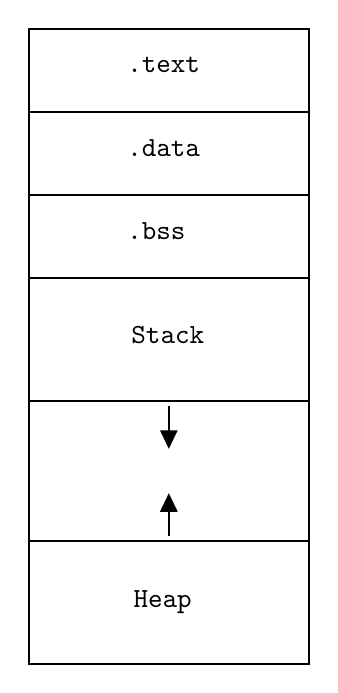
\begin{tikzpicture}[x=0.75pt,y=0.75pt,yscale=-1,xscale=1]
%uncomment if require: \path (0,339); %set diagram left start at 0, and has height of 339

%Shape: Rectangle [id:dp13101589938105973] 
\draw   (243,10) -- (378,10) -- (378,50) -- (243,50) -- cycle ;
%Shape: Rectangle [id:dp06368153206435134] 
\draw   (243,50) -- (378,50) -- (378,90) -- (243,90) -- cycle ;
%Shape: Rectangle [id:dp8533115917784224] 
\draw   (243,90) -- (378,90) -- (378,130) -- (243,130) -- cycle ;
%Shape: Rectangle [id:dp04455868614862735] 
\draw   (243,130) -- (378,130) -- (378,189.2) -- (243,189.2) -- cycle ;
%Shape: Rectangle [id:dp9354652197962545] 
\draw   (243,257) -- (378,257) -- (378,316.2) -- (243,316.2) -- cycle ;
%Straight Lines [id:da9885326185507459] 
\draw    (243,189.2) -- (243,257) ;
%Straight Lines [id:da5770026001630877] 
\draw    (378,189.2) -- (378,257) ;
%Straight Lines [id:da33638011482323815] 
\draw    (310.5,191.6) -- (310.5,209.4) ;
\draw [shift={(310.5,212.4)}, rotate = 270] [fill={rgb, 255:red, 0; green, 0; blue, 0 }  ][line width=0.08]  [draw opacity=0] (8.93,-4.29) -- (0,0) -- (8.93,4.29) -- cycle    ;
%Straight Lines [id:da3195032750258344] 
\draw    (310.5,236.8) -- (310.5,254.6) ;
\draw [shift={(310.5,233.8)}, rotate = 90] [fill={rgb, 255:red, 0; green, 0; blue, 0 }  ][line width=0.08]  [draw opacity=0] (8.93,-4.29) -- (0,0) -- (8.93,4.29) -- cycle    ;

% Text Node
\draw (289,22) node [anchor=north west][inner sep=0.75pt]   [align=left] {\texttt{.text}};
% Text Node
\draw (289,62) node [anchor=north west][inner sep=0.75pt]   [align=left] {\texttt{.data}};
% Text Node
\draw (289,102) node [anchor=north west][inner sep=0.75pt]   [align=left] {\texttt{.bss}};
% Text Node
\draw (291,152) node [anchor=north west][inner sep=0.75pt]   [align=left] {\texttt{Stack}};
% Text Node
\draw (292,279) node [anchor=north west][inner sep=0.75pt]   [align=left] {\texttt{Heap}};


\end{tikzpicture}
    \caption{Vanlig minne-struktur for et program.}
    \label{fig:4-minne-struktur}
\end{figure}

Feltet \verb|.data| og \verb|.bss| inneholder henholdsvis \textit{compile time} initialisert-allokert og uinitialisert minne. Disse feltene er for globale variabler.

\verb|Heap|-feltet er området minne-kall til \verb|malloc| og \verb|free| vil virke på. \verb|Heap|-en er for dynamisk allokert minne, og vil vokse oppover dersom en gjennom kall til \verb|malloc| bruker opp allokert \verb|heap|-størrelse.

Ovenfor \verb|heap|-en ligger området for \verb|stack|-en. Denne vil bestå av såkalte \verb|stack|-frames med lokale variabler. Om du gjør uendelig rekursjon i et språk som ikke støtter \textit{tail recursion}, så vil \verb|stack|-en vokse nedover til den til slutt kolliderer med \verb|heap|-en. Dette er det som kalles en \textit{stack overflow}.

Nøyaktig hvor dynamisk lenkede biblioteker ligger, og hvor kopier av eksterne variabler finnes, er implementasjonsspesifikt - men de generelle trekkene i figur \ref{fig:4-minne-struktur} stemmer som regel.

Når dere kjører et program vil dere som regel ikke jobbe direkte med informasjon som er lagret på harddisk eller annet sekundærminne. Grunnen til dette er at både skriving til og lesing fra datamaskinens primærminne som ofte består av RAM (\textbf{R}andom \textbf{A}ccess \textbf{M}emory) er betydelig raskere enn til og fra harddisken. Under kjøring av et program laster derfor datamaskinen deler av informasjon fra sekundærminne til primærminne, altså typisk fra harddisk til RAM. Disse delene kalles \textit{memory pages}, og størrelsen på disse er avhengig av arkitektur. Operativsystemet vil gi hver \textit{memory page} diverse flagg for å holde styr på hva man kan gjøre med minnet.

Uheldigvis er det ganske vanlig at man har et array som ikke tar en hel \textit{page}. Dermed kan man gjøre ulovlige minne-operasjoner så lenge man er `heldig' og treffer en \textit{page} som man har aksess-rettigheter til. En \textit{out-of-bounds} på ett element vil derfor ikke alltid gi en segfault, som det burde.

\section{Appendiks - Windows Subsystem for Linux (WSL)}\label{app:wsl}
Windows Subsystem for Linux (WSL) er en snedig måte å kjøre Linux på Windows uten å ha en ekstra partisjon på harddisken. Tidligere var såkalte \textit{virtual boxes} en populær måte å kjøre Linux på Windows på, men på grunn av dårlig ytelse blir dette lite brukt i dag. WSL gir deg muligheten til å kjøre en valgfri Linux-distribusjon fra terminalen uten noe særlig \textit{overhead}, og detta er jo stas! Stegene som presenteres i denne guiden er hentet \href{https://learn.microsoft.com/en-us/windows/wsl/install}{herfra}.

\begin{enumerate}
    \item Trykk \verb|Windows + R|
    \item Skriv inn \verb|cmd| og trykk \verb|Enter|
    \item Skriv inn \verb|wsl --install| i terminalen og trykk \verb|Enter|
\end{enumerate}

Det var alt som trengtes for å installere WSL. Hvis du nå vil bruke Ubuntu trenger du bare å skrive \verb|ubuntu| i Windows-terminalen og trykke \verb|Enter|. Det er også mulig å installere andre distribusjoner enn \verb|Ubuntu|, men som sagt er dette distribusjonen som brukes på Sanntidssalen, og vi velger derfor denne her.

\section{Appendiks - VSCode og WSL}\label{app:wsl+vscode}
Når WSL er installert på Windows kan man åpne det gjennom å skrive \verb|ubuntu| i \verb|Command Prompt| eller \verb|PowerShell|. Deretter følger vi \href{https://code.visualstudio.com/docs/setup/linux}{denne guiden} for å installere VSCode i WSL. Dersom man allerede har VSCode installert på Windows-maskina, så har man også muligheten til å kjøre det gjennom WSL, og man trenger ikke laste det ned på nytt, og dette anbefales også. Har man derimot ikke VSCode installert, kan man gjøre følgende steg for å installere det manuelt:

\begin{lstlisting}[language=bash]
sudo apt-get install wget gpg

wget -qO- https://packages.microsoft.com/keys/microsoft.asc | gpg --dearmor > packages.microsoft.gpg

sudo install -D -o root -g root -m 644 packages.microsoft.gpg /etc/apt/keyrings/packages.microsoft.gpg

sudo sh -c 'echo "deb [arch=amd64,arm64,armhf signed-by=/etc/apt/keyrings/packages.microsoft.gpg] https://packages.microsoft.com/repos/code stable main" > /etc/apt/sources.list.d/vscode.list'

rm -f packages.microsoft.gpg
\end{lstlisting}

Deretter oppdaterer du pakke-\textit{cachen}, og og installerer pakken ved bruk av:

\begin{lstlisting}[language=bash]
sudo apt install apt-transport-https

sudo apt update

sudo apt install code # or code-insiders
\end{lstlisting}

Nå som du har VSCode, kan du bruke det gjennom WSL ved å skrive \verb|code .| i terminalen, for å åpne brukergrensesnittet i den mappen du nå befinner deg i. Dersom du ønsker å åpne en mappe eller fil i VSCode direkte kaller du \verb|code name|, der "name" byttes ut med navnet til filen eller mappa. Nå kjøres VSCode gjennom WSL, men det grafiske brukergrensesnittet minner veldig om slik det ville sett ut dersom det ble kjørt direkte fra Windows. Her får du imidlertid tilgang til et liknende miljø som på PCene i Sanntidssalen, og det er nøyaktig derfor vi presenterer denne måten å jobbe på.

Det skal også nevnes at det kan være nyttig å laste ned \verb|WSL|-utvidelsen til VSCode. For å gjøre dette, trykk \verb|Ctrl + Shift + X| i VSCode for å åpne utvidelses-fanen, og søk på \verb|WSL| for å finne riktig utvidelse. Last ned denne.

Dersom man av en eller annen grunn skulle få lyst til å avinstallere VSCode fra WSL, kan man bruke følgende kommando: \verb|sudo apt-get remove code|.

\section{Appendiks - C/C++ i VSCode for WSL}\label{app:C_VSCode_WSL}
For å kunne kompilere kode i VSCode for WSL, så er vi avhengige av riktig oppsett for kompilatoren og debuggeren vi skal bruke. Som dere er kjent med fra tidligere i denne øvingen skal vi bruke \verb|GCC| for å kompilere C/C++-kode, samt \verb|GDB| for debugging. Guiden vi skal følge er \href{https://code.visualstudio.com/docs/cpp/config-wsl}{denna her}.

\begin{enumerate}
    \item Kjør \verb|sudo apt-get update|.
    \item Kjør \verb|sudo apt-get install build-essential gdb|.
    \item Sjekk at \verb|GDB| og \verb|GCC| er riktig installert ved kommandoene \verb|whereis gdb| og \verb|whereis gcc|. Dersom filplasseringene returneres bekrefter dette at installasjonene var vellykkede.
\end{enumerate}

Nå som dere har \verb|GCC| og \verb|GDB| installert er dere i stand til å både kjøre og debugge C/C++-kode i VSCode. Hvordan dette gjøres lærer dere i avsnitt \ref{sec:debugging}.